% !TEX root = _main.tex

\begin{figure*}[tb]
	\centering
	\begin{minipage}{0.36\hsize}
		\centering
		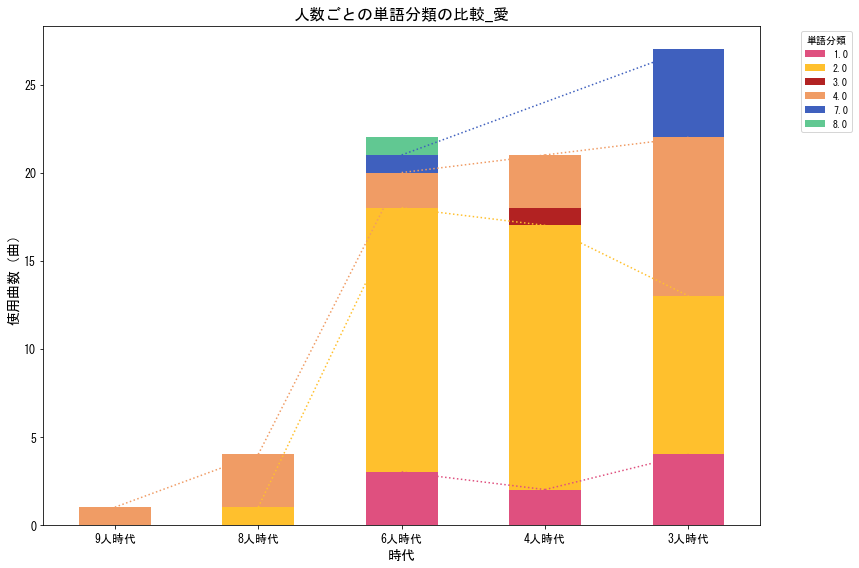
\includegraphics[width=\hsize]{fig/ai-ninzu.png}
		\caption{「愛」人数時代別使用意味比較}
		\label{fig:ai-ninzu}
	\end{minipage}
	\begin{minipage}{0.62\hsize}
		\centering
		\scriptsize
		\captionof{table}{「愛」人数別時代ごとの\kyokusu （()内は割合）}
		\label{tab:ai-uchi}
		\begin{tabular}{c|cccccc}
			\hline
			「愛」の分類 & ９人時代      & ８人時代     & ６人時代      & ４人時代      & ３人時代      & 合計        \\
			\hline\hline
			1:家族愛  & 0 (0.0)   & 0 (0.0)  & 3 (13.6)  & 2 (9.5)   & 4 (14.8)  & 9 (12.0)  \\
			2:性愛   & 0 (0.0)   & 1 (25.0) & 15 (68.2) & 15 (71.4) & 9 (33.3)  & 40 (53.3) \\
			3:大切な愛 & 0 (0.0)   & 0 (0.0)  & 0 (0.0)   & 1 (4.8)   & 0 (0.0)   & 1 (1.3)   \\
			4:壮大な愛 & 1 (100.0) & 3 (75.0) & 2 (9.1)   & 3 (14.3)  & 9  (33.3) & 18 (24.0) \\
			7:韻表現  & 0 (0.0)   & 0 (0.0)  & 1 (4.5)   & 0 (0.0)   & 5 (18.5)  & 6 (8.0)   \\
			8:その他  & 0 (0.0)   & 0 (0.0)  & 1 (4.5)   & 0 (0.0)   & 0 (0.0)   & 1 (1.3)   \\
			\hline
			合計     & 1         & 4        & 22        & 21        & 27        & 75        \\
			\hline
		\end{tabular}
	\end{minipage}
\end{figure*}